	\documentclass[10pt,oneside]{CBFT_book}
	% Algunos paquetes
	\usepackage{amssymb}
	\usepackage{amsmath}
	\usepackage{graphicx}
	\usepackage{libertine}
	\usepackage[bold-style=TeX]{unicode-math}
	\usepackage{lipsum}

	\usepackage{natbib}
	\setcitestyle{square}

	\usepackage{polyglossia}
	\setdefaultlanguage{spanish}


	\usepackage{CBFT.estilo} % Cargo la hoja de estilo

	% Tipografías
	% \setromanfont[Mapping=tex-text]{Linux Libertine O}
	% \setsansfont[Mapping=tex-text]{DejaVu Sans}
	% \setmonofont[Mapping=tex-text]{DejaVu Sans Mono}

	%===================================================================
	%	DOCUMENTO PROPIAMENTE DICHO
	%===================================================================

\begin{document}

% =================================================================================================
\chapter{Expansión en un campo multipolar}
% =================================================================================================

% =================================================================================================
\section{Desarrollo dipolar del campo magnético}
% =================================================================================================

El potencial vector de un dipolo es
\[
	\vb{A}(\vb{x}) = \frac{\vb{v}\times(\vb{x}-\vb{x}')}{|\vb{x}-\vb{x}'|^3} = \vb{m} \times \Nabla 
		\frac{1}{|\vb{x}-\vb{x}'|}
\]
\[
	\vb{A}(\vb{x}) = \int_{V'} \vb{\mathcal{M}}(\vb{x}') \times \Nabla 
			\left(\frac{1}{|\vb{x}-\vb{x}'|}\right) dV'
\]
Es el potencial vector de una distribución de momento dipolar magnético con densidad $ \vb{M}(\vb{x}')$

\[
	\vb{A}(\vb{x}) = \int_{V'} \frac{\rotorm{\vb{M}}}{|\vb{x}-\vb{x}'|} dV' +
			\int_{S'} \frac{\vb{M}\times\hat{n}}{|\vb{x}-\vb{x}'|} dS'
\]
y se pueden pensar como corrientes $\vb{J}_M$ y $\vb{g}_M$,
\[
	\vb{A}(\vb{x}) = \frac{1}{c} \int_{V'} \frac{\vb{J}_M}{|\vb{x}-\vb{x}'|} dV' +
			\frac{1}{c} \int_{S'} \frac{\vb{g}_M}{|\vb{x}-\vb{x}'|} dS'
\]

% =================================================================================================
\section{Medios materiales}
% =================================================================================================

\begin{itemize}
 \item Dieléctricos
 \item Medios magnéticos
	$\begin{cases}
	 \text{imán inducido}
		\begin{cases}
		\text{paramagnético} \\
		\text{diamagnético}
		\end{cases} \\
	 \text{imán permanente} \quad \text{ferromagnético}
	\end{cases}$
 \item Conductor
	$\begin{cases}
	 \text{perfecto} \\
	 \text{buen conductor} \\
	 \text{mal conductor}
	\end{cases}$
\end{itemize}

Podemos hacer una suerte de tabla comparativa entre eléctrico y magnético
(pero lo armaremos después con minipage)

Polarización  
\[
	\vb{P} = \frac{\delta \vb{p}}{\delta V}
\]
que es el Momento dipolar eléctrico por unidad de volumen. Luego el potencial es
\[
	\phi( \vb{x}) = \int_S \frac{\vb{P}(\vb{x}')}{|\vb{x}-\vb{x}'|} d\vb{S}' - 
	\int_V \frac{\Nabla\cdot\vb{P}(\vb{x}')}{|\vb{x}-\vb{x}'|}  dV'
\]
\[
	\qquad \vb{P}\cdot\hat{n} = \sigma_P \qquad \Rightarrow \qquad \divem{P} = -\rho_0
\]
\[
	\begin{cases}
	\rotorm{E}  = 0 \\
	\divem{E} = 4\pi\rho = 4\phi( \rho_L + \rho_P )
	\end{cases}
\]
\[
	\divem{E} -  4\phi\rho_P = 4\phi\rho_L 
\]
\[
	\divem{E} + 4 \pi \divem{P} = \Nabla\cdot(\vb{E} + 4\pi\vb{P} )
\]
de modo que
\[
	\vb{D} = \vb{E} + 4 \pi \vb{P} \qquad \qquad \divem{D} = 4\pi\rho_L
\]
y por la linealidad
\[
	\vb{P} = \xi_e \vb{E} \qquad \text{MLIH}
\]
\[
	\vb{D} = ( 1 + 4\pi\xi_e ) \vb{E} 
\]
\[
	\vb{D} = \epsilon \vb{E}
\]
donde $\xi_e$ es la susceptibilidad eléctrica y $\epsilon$ es la permitividad eléctrica.
Los contornos entre medios se resuelven según
\[
	\hat{n} \times (\vb{E}_2 -\vb{E}_1) = 0 \qquad 
	(\vb{D}_2 -\vb{D}_1)\cdot\hat{n} = 4 \pi \sigma_L \qquad 
	(\vb{P}_2 -\vb{P}_1)\cdot\hat{n} = - \sigma_L
\]

Para la Magnetización,
\[
	\vb{M} = \frac{\delta \vb{m}}{\delta V}
\]
que es el Momento dipolar magnético por unidad de volumen. Luego el potencial es
\[
	\vb{A}( \vb{x}) = \frac{1}{c} \int_S \frac{ \vb{M}\times\hat{n} }{|\vb{x}-\vb{x}'|} d\vb{S}' - 
	\frac{1}{c} \int_V \frac{ c(\rotorm{M}) }{|\vb{x}-\vb{x}'|}  dV'
\]
\[
	\rotorm{M} = \frac{1}{c}\vb{J}_M \qquad \qquad \vb{M}\times\hat{n} = \frac{1}{c}\vb{g}_m
\]
\[
	\rotorm{B} = \frac{4\pi}{c}\vb{J}  = \frac{4\pi}{c}( \vb{J}_L + \vb{J}_M )
\]
\[
	\rotorm{B} - 4\pi \rotorm{M} = \frac{4\pi}{c}\vb{J}_L
\]
\[
	\Nabla\times( \vb{B} - 4\pi\vb{M} ) = \frac{4\pi}{c}\vb{J}_L 
\]
de modo que
\[
	\vb{H} = \vb{B} - 4 \pi \vb{M} \qquad \qquad \divem{M} = \frac{1}{c}\vb{J}_M  
\]
y por la linealidad
\[
	\vb{M} = \xi_M \vb{H} \qquad \text{MLIH}
\]
\[
	\vb{B} = ( 1 + 4\pi\xi_M ) \vb{H} 
\]
\[
	\vb{B} = \epsilon \vb{H}
\]
donde $\xi_M$ es la susceptibilidad magnética y $\mu$ es la permeabilidad magnética.
Los contornos entre medios se resuelven según
\[
	\hat{n} \times (\vb{H}_2 -\vb{H}_1) = \frac{4 \pi}{c} \vb{g}_L \qquad 
	(\vb{B}_2 -\vb{B}_1)\cdot\hat{n} = 0 
\]

\subsubsection{Imán permanente}

Hay magnetización \vb{M} aún en ausencia de campo. No es un medio lineal de modo que
\[
	\vb{M}	 \neq \xi_M \vb{H} \Rightarrow \vb{B} \neq \mu \vb{H}
\]
La relación entre \vb{B},\vb{H} depende de la historia del medio.
\[
	\frac{1}{c}\vb{J}_M = \rotorm{M}
\]
si \vb{J}$_L=0$ entonces 
\[
	\rotorm{H} = 0 \qquad \Rightarrow \vb{H} = -\Nabla\phi_m
\]
que es un potencial escalar magnético.
\[
	\Nabla\cdot( \vb{H} + 4\pi\vb{M} ) = \divem{B} = 0
\]
\[
	\divem{H} = -4\pi\divem{M}
\]
\[
	-\nabla^2 \phi_m = -4\pi\divem{M}
\]
\[
	\nabla^2 \phi_m = -4\pi\rho_m
\]
\[
	\divem{M} \equiv -\rho_m \qquad \qquad \vb{M}\cdot\hat{n} \equiv \sigma_m
\]
\[
	\phi_m = \frac{1}{c} \int_{S'} \frac{\vb{M}}{|\vb{x}-\vb{x}'|} \cdot d\vb{S}' -
		\frac{1}{c} \int_{V'} \frac{\divem{M}}{|\vb{x}-\vb{x}'|} dV' 
\]
\[
	\vb{A}( \vb{x}) = \frac{1}{c} \int_S \frac{ \vb{M}\times\hat{n} }{|\vb{x}-\vb{x}'|} d\vb{S}' - 
		\frac{1}{c} \int_V \frac{ c(\rotorm{M}) }{|\vb{x}-\vb{x}'|}  dV'
\]
Estas dos soluciones son equivalentes.
\[
	\phi_m = \frac{1}{c} \int_{V'} \frac{\rho_L}{|\vb{x}-\vb{x}'|}  dV' +
		\frac{1}{c} \int_{V'} \frac{ \vb{P}\cdot(\vb{x}-\vb{x}')}{|\vb{x}-\vb{x}'|^3} dV' 
\]
pero el integrando del segundo término se puede reescribir como 
\[
	-\vb{P}\cdot\Nabla\left(\frac{1}{|\vb{x}-\vb{x}'|}\right)
\]
de manera que 
\[
	\phi_m = \frac{1}{c} \int_{V'} \frac{\rho_L}{|\vb{x}-\vb{x}'|}  dV' -
		\frac{1}{c} \int_{V'} \frac{ \divem{P}) }{|\vb{x}-\vb{x}'|} dV' 
\]
\[
	\phi_m = \frac{1}{c} \int_{V'} \frac{1}{|\vb{x}-\vb{x}'|}( \rho - \divem{P} )  dV'
\]
se puede asociar
\[
	\divem{P} = \rho_P.
\]

\[
	\vb{A}( \vb{x}) = \frac{1}{c} \int_V \left[ \frac{ \vb{J}_L(\vb{x}') }{|\vb{x}-\vb{x}'|} +
		\frac{ c \vb{M} \times (\vb{x}-\vb{x}') }{|\vb{x}-\vb{x}'|^3} \right] dV'
\]
\[
	\vb{A}( \vb{x}) = \frac{1}{c} \int_V \left[ \frac{ \vb{J}_L(\vb{x}') }{|\vb{x}-\vb{x}'|} +
		\frac{ c \divem{M} }{|\vb{x}-\vb{x}'|} \right] dV'
\]
\[
	\vb{A}( \vb{x}) = \frac{1}{c} \int_V \frac{ \vb{J}_L(\vb{x}') + \vb{J}_M(\vb{x}' ) }{|\vb{x}-\vb{x}'|}	
\]

\begin{figure}[htb]
	\begin{center}
	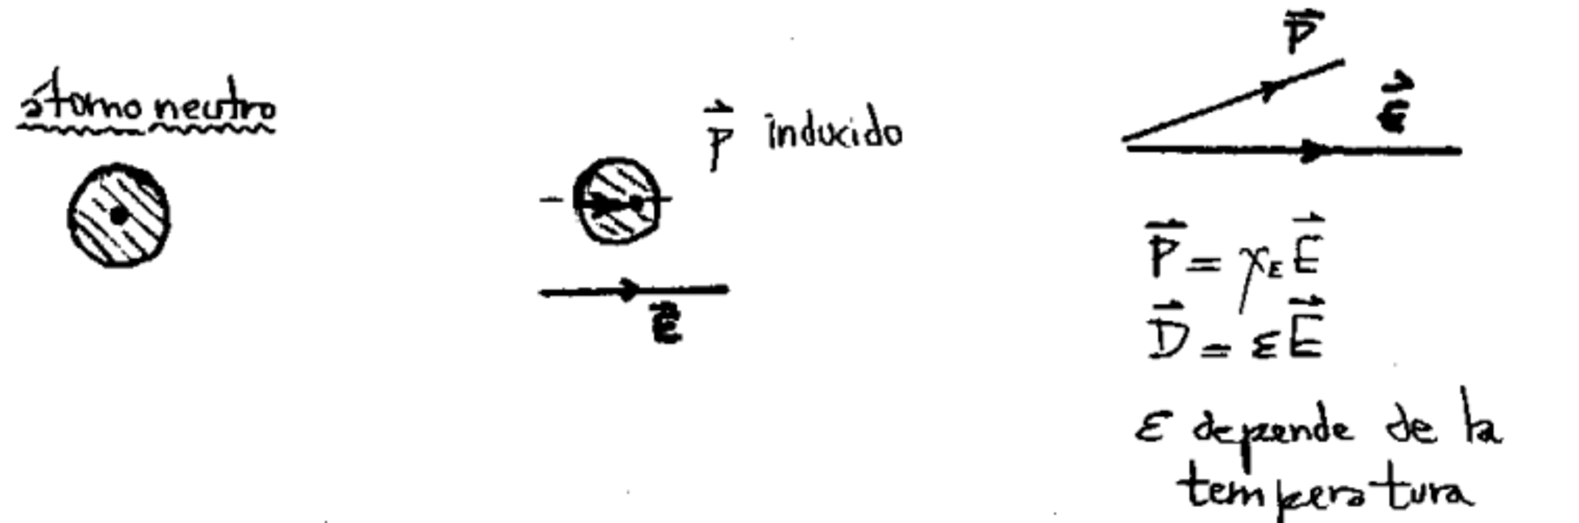
\includegraphics[width=0.6\textwidth]{images/fig_ft1_magnetizaciones.pdf}	 
	\end{center}
	\caption{}
\end{figure}


% =================================================================================================
\section{Polarización y magnetización}
% =================================================================================================

Suelen \vb{P},\vb{M} depender de los campos externos, es decir $\vb{P}=\vb{P}(\vb{E})$ y 
$\vb{M}=\vb{M}(\vb{H})$.
\[
	\vb{M} \approx M_{0i} + \left.\dpar{M_i}{H_j}\right|_{H=0} H_j
\]
\[
	\vb{P} \approx P_{0i} + \left.\dpar{P_i}{E_j}\right|_{E=0} E_j
\]
y como en general vale que $\vb{M}_0=0, \vb{P}_0=0$  se da que 
\[
	\vb{M} = \sum_i \sum_j \left( \left.\dpar{M_i}{H_j}\right|_{H=0} H_j \right) 
\]
\[
	\vb{M} = 
	\begin{pmatrix}
	 \displaystyle{\dpar{M_x}{H_x}} & \displaystyle{\dpar{M_x}{H_y}} & \displaystyle{\dpar{M_x}{H_z}} \\
	 \displaystyle{\dpar{M_y}{H_x}} & \displaystyle{\dpar{M_y}{H_y}} & \displaystyle{\dpar{M_y}{H_z}} \\
	 \displaystyle{\dpar{M_z}{H_x}} & \displaystyle{\dpar{M_z}{H_y}} & \displaystyle{\dpar{M_z}{H_z}}
	\end{pmatrix}
	\begin{pmatrix}
	 \displaystyle{H_x} \\
	 \\
	 H_y \\
	 \\
	 H_z
	\end{pmatrix}
\]
y ahí vemos que es un tensor,
\[
	\vb{M} = \overleftrightarrow{\xi}_M \vb{H} \qquad\qquad \vb{P} =  \overleftrightarrow{\xi}_e \vb{E}.
\]

\subsubsection{Algún detalle de contornos magnéticos}

\begin{figure}[htb]
	\begin{center}
	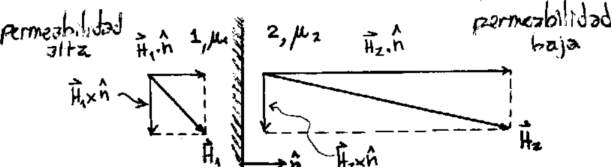
\includegraphics[width=0.6\textwidth]{images/fig_ft1_medios1.pdf}	 
	\end{center}
	\caption{}
\end{figure}
Sea
\[
	\vb{g}_L = 0 
\]
entonces
\[
	\hat{n}\times\vb{H}_1 = \hat{n}\times\vb{H}_2
\]
\[
	\vb{B}_1\cdot\hat{n} = \vb{B}_2\cdot\hat{n} \qquad
		\mu_1\vb{H}_1\cdot\hat{n} = \mu_2\vb{H}_2\cdot\hat{n}
\]
\[
	H_2 = \frac{\mu_1}{\mu_2} H_1 \quad \text{si} \; \mu_1 \gg \mu_2 \Rightarrow H_2 \gg H_1
\]
En el límite $\vb{H}_2 \perp$ superficie del medio y es similar al \vb{E} a la salida de un
conductor; las superficies de materiales de permeabilidad muy alta son aproximadamente {\it equipotenciales}.

Para medio anisótropo
\[
	D_i = \epsilon_{ij} E_j \qquad \text{es decir} \quad \vb{D} = \overleftrightarrow{\epsilon} \vb{E}
\]

\subsubsection{Consideraciones en medios magnéticos}

Fuera de un imán permanente 
\[
	\rotorm{B} = 0 = \frac{4\pi}{c}\vb{J}_T
\]
y entonces parecería que podemos definir un
\[
	\vb{B} = -\Nabla \phi_m^B,
\]
pero fallará en la superficie de separación donde hay \vb{J}$_m$ y por ende \vb{J}$_T$. Lo que sí funciona
es
\[
	\rotorm{H} = 0 = \frac{4\pi}{c}\vb{J}_L
\]
que vale dentro y fuera del imán.
\begin{figure}[htb]
	\begin{center}
	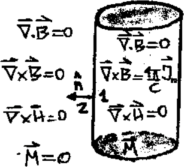
\includegraphics[width=0.25\textwidth]{images/fig_ft1_medios2.pdf}	 
	\end{center}
	\caption{}
\end{figure}

Entonces
\[
	\vb{H} = -\Nabla \phi_m^H,
\]
y
\[
	\divem{H} = -\Nabla(\Nabla \phi^H_m ) = -4\pi \divem{M} = 4\pi\rho_M
\]
\[
	-\nabla^2 \phi_m^H = 4\pi\rho_M
\]
una ecuación de Poisson para el potencial $\phi_m^H$.

\[
	(\vb{B}_2 - \vb{B}_1)\cdot\hat{n} = 0
\]
\[
	(-\Nabla \phi^2_H + \Nabla \phi^1_H - 4\pi \vb{M})\cdot\hat{n} = 0
\]
\[
	(-\Nabla \phi^2_H + \Nabla \phi^1_H )\cdot\hat{n} = 4\pi \vb{M}\cdot\hat{n} = 4\pi \sigma_M
\]

% =================================================================================================
\section{Consideraciones energéticas}
% =================================================================================================

\[
	\vb{F} = q \vb{E} = q (-\Nabla\phi) = - \Nabla U
\]
\[
	\Delta U = W = \int_\Gamma \vb{F}\cdot d\vb{\ell} \rightarrow \Delta U = 
	- \int_\Gamma \Nabla (q\phi) \cdot d\vb{\ell} = -q \Delta \phi
\]
\[
	\delta U = \vb{F}\cdot\delta\vb{x} \qquad\qquad  \frac{\delta U}{\delta x} = F_t
\]
donde el subíndice es por tangencial.
\[
	W_2 = q_2 \frac{q_1}{r_{12}} = \frac{1}{2}\left( q_1 \frac{q_2}{r_{12}} + 
		q_2 \frac{q_1}{r_{21}} \right)
\]
\[
	W_3 = q_2 \frac{q_1}{r_{12}} + q_3 \frac{q_1}{r_{13}} + q_2 \frac{q_3}{r_{23}}
\]
\[
	W_3 = \frac{1}{2}\left( q_1 \frac{q_2}{r_{12}} + q_1 \frac{q_3}{r_{13}} + q_2 \frac{q_1}{r_{21}}
		+ q_2 \frac{q_3}{r_{23}} + q_3 \frac{q_1}{r_{31}} + q_3 \frac{q_2}{r_{32}} \right)
\]
\[
	W_N = \sum_{i\neq j}^N \frac{1}{2}\frac{q_i q_j}{r_{ij}} =
	\sum_{i,j}^N \frac{1}{2} q_i \phi_{ij}[ 1 - \delta_{ij}]
\]
siendo $\phi_{ij}$ el potencial sobre $q_i$ debido a $q_j$.
\[
	W_N = \sum_i^N \frac{1}{2} q_i \phi_i 
\]
es el potencial de todas las cargas producido en la posición de $q_i$.
\[
	W = \frac{1}{2} \int_V \rho(\vb{x}) \phi(\vb{x}) dV
\]
Supongamos ahora la presencia de un medio material 
\[
	\delta W = \frac{1}{2} \rho \delta V \phi
\]
\[
	\delta W = \frac{1}{2}\frac{\Nabla\cdot(\delta\vb{D})}{4\pi} \delta V \phi 
\]
\[
	\Nabla\cdot(\delta\vb{D}\phi) = \delta\vb{D} \cdot \Nabla\phi  + \phi \Nabla\cdot\delta\vb{D}
\]
\[
	\delta W = \frac{1}{8\pi} \delta V [\Nabla\cdot(\delta\vb{D}\phi) - \delta\vb{D} \cdot \Nabla\phi ]
\]
\[
	W = \frac{1}{8\pi}\left( \int_V \Nabla\cdot(\vb{D}\phi)dV + \int_V \vb{D}\cdot\vb{E} dV \right)
\]
pero la primera integral se pasa a una de superficie según
\[
	\int_S \vb{D}\phi dS
\]
y si la misma es muy grande tiende a cero. Entonces quedamos en que 
\[
	W = \frac{1}{8\pi} \int_V \vb{D}\cdot\vb{E} dV
\]
que es el trabajo necesario para formar una configuración en presencia de medios materiales. Vale
para medios lineales, sin imponer isotroía u homogeneidad.

Este cálculo es a temperatura constante, el medio material no altera su $\epsilon$.
Es un proceso isotérmico. Uno asume que $\epsilon=\epsilon(\vb{x})$ y no varía con el tiempo.
En la práctica $\epsilon$ varía con la temperatura.

% =================================================================================================
\section{Interpretación termodinámica de U}
% =================================================================================================

El incremento de energía a T constante
\be
	\delta W = U = \frac{1}{8 \pi} \vb{E}\cdot\vb{D} = \frac{1}{8 \pi} \epsilon_{ij}E_i E_j	\qquad
	\text{con} \; \epsilon_{ij} = \epsilon_{ji} \; \text{tensor simétrico}
	\label{energíaEM}
\ee
Pero $\epsilon$ es función de T la temperatura y entonces no podemos decir que
\[
	dU = dW
\]
valga en general, pues también hay variación del calor (a no ser que sea un proceso isotérmico) de modo que 
la energía que representa \eqref{energíaEM} es la energía libre de Helmholtz a T constante.
\[
	dU = dQ - dW \qquad \qquad F = U - TS
\]
\[
	dF = dU - TdS - SdT
\]
pero al ser la última cero, resulta
\[
	dF|_T = dU - T.dS = \frac{1}{8\pi} \int_V \vb{E}\cdot\delta\vb{D} dV
\]
\[
	dF = \frac{1}{8\pi} \int_V \vb{E}\cdot\delta\vb{D} dV - SdT
\]
de modo que como el primer término es $\partial F / \partial D |_T$ resulta que 
\[
	S = -\left.\dpar{F}{T}\right|_D
\]

Si es un medio isótropom entonces $\vb{D} = \epsilon \vb{E}$ y entonces 
\[
	F = \frac{1}{8\pi} \int_V \frac{1}{\epsilon}\vb{D}\cdot\vb{D} dV
\]
entonces
\[
	\left.\dpar{F}{T}\right|_D	= \frac{1}{8\pi} \int_V \vb{D}\cdot\vb{D} \frac{\partial}{\partial T}
		\left( \frac{1}{\epsilon} \right) dV
\]
\[
	=  - \frac{1}{8\pi} \int_V \vb{D}\cdot\vb{D} \frac{1}{\epsilon^2} \dpar{\epsilon}{T}  dV =
	-\frac{1}{8\pi} \int_V \vb{E}\cdot\vb{D} \frac{1}{\epsilon} \dpar{\epsilon}{T}  dV = S
\]
luego 
\[
	U = F + TS = \frac{1}{8\pi} \int_V \vb{D}\cdot\vb{D} \frac{1}{\epsilon} dV  +
	\frac{1}{8\pi} \int_V \vb{E}\cdot\vb{D} \frac{1}{\epsilon} \dpar{\epsilon}{T}  dV 
\]
\[
	U = \frac{1}{8\pi} \int_V \frac{1}{\epsilon} \left[ \vb{D}\cdot \left( \vb{D} + 
		\vb{E} \dpar{\epsilon}{T} T \right) \right] dV  = \frac{1}{8\pi} \int_V \frac{1}{\epsilon}
		\vb{D}\cdot \vb{E} \left[ \epsilon + T \dpar{\epsilon}{T}  \right] dV
\]
y finalmente para medios lineales e isótropos
\[
	U = \frac{1}{8\pi} \int_V \frac{1}{\epsilon} \vb{D}\cdot \vb{E} \dpar{ T \epsilon}{T} dV
\]
y la segunda ley de la termodinámica es
\[
	\delta Q = T.dS = \frac{1}{4\pi} \int_V \vb{E}\cdot\delta\vb{D} \frac{T}{\epsilon}
	\dpar{\epsilon}{T} dV
\]
con $\epsilon > 0, T > 0, \partial \epsilon / \partial T < 0$ si el $\epsilon$ decrece con T el cuerpo
se enfría $\delta Q < 0$.







% \bibliographystyle{CBFT-apa-good}	% (uses file "apa-good.bst")
% \bibliography{CBFT.Referencias} % La base de datos bibliográfica

\end{document}
